\section{Випадковий ліс}

Алгоритм машинного навчання, який називається випадковий ліс, --- це
своєрідний оцінювач, який підходить до ряду класифікуючих дерев рішень
на різних гілках набору даних і використовує усереднення для підвищення
точності прогнозування та контролю над вхідною інформацією.

В основі алгоритму випадкового лісу (рис. \ref{fig:random-forest}) лежать так звані
дерева рішень, за допомогою яких відбувається обробка вхідної інформації.
У машинному навчанні дерева рішень --- це метод для обчислення
значень та параметрів моделі у прогнозуванні. Цю назву вони отримали,
тому що прийняття рішень та вихідний результат будуються за гілками: таким чином
створюється ніби дерево, де кожна гілка відповідає на питання ``якщо ...
тоді ...'' --- подібно до гілок дерева.

Якщо ми уявимо, що ми почнемо з певної вибірки, для якої ми хочемо
передбачити клас чи побудувати регресійну модель, то потрібно починати з
низу гілки і йти за рішеннями вгору, щоб отримати відповідь, поки не
дійдемо до першої розгалуженої гілки. Це розгалуження можна вважати
особливістю цього методу машинного навчання, і питання в тому, де вона
з’явиться. Далі йде послідовне прийняття рішень щодо того, чи йти далі,
чи обрати іншу гілку для обробки рішень. Це відбувається доти, доки
не приймається рішення про перехід на наступну гілку, або повторити
процес знову, тим самим покращивши результати. Ця кінцева точка
називається аркушем, і в деревах рішень представлений кінцевий
результат: передбачуваний клас або значення.

\begin{figure}[H]
  \centering
  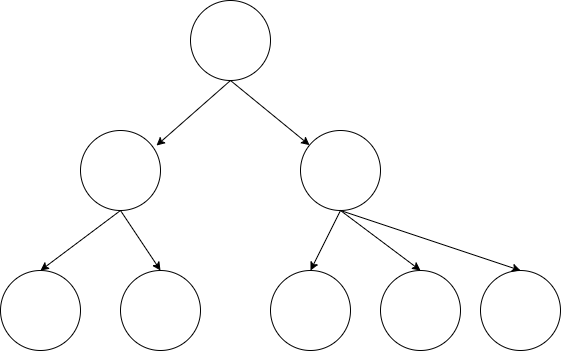
\includegraphics[width=0.7\textwidth]{images/image17}
  \caption{Приклад ансамблю дерев}
  \label{fig:random-forest}
\end{figure}
